 \documentclass[11pt,a4paper]{article}
\usepackage[utf8]{inputenc}		% LaTeX, comprend les accents !
\usepackage[T1]{fontenc}
\usepackage{natbib}	
%\usepackage[square,sort&compress,sectionbib]{natbib}		% Doit être chargé avant babel      
\usepackage[frenchb,english]{babel}
\usepackage{lmodern}
\usepackage{amsmath,amssymb, amsthm}
\usepackage{a4wide}
\usepackage[capposition=top]{floatrow}
\usepackage{verbatim}
\usepackage{float}
\usepackage{placeins}
\usepackage{flafter}
\usepackage{longtable}
\usepackage{import}
\usepackage{pdflscape}
\usepackage{rotating}
\usepackage{hhline}
\usepackage{multirow}
\usepackage{booktabs}
\usepackage[pdftex,pdfborder={0 0 0},colorlinks=true,linkcolor=blue,urlcolor=blue,citecolor=blue,bookmarksopen=true]{hyperref}
\usepackage{eurosym}
%\usepackage{breakcites}
\usepackage[autostyle]{csquotes}
%\usepackage{datetime}
\usepackage{natbib}
\usepackage{setspace}
\usepackage{lscape}
\usepackage[usenames]{color}
\usepackage{indentfirst}
\usepackage{url}
\usepackage{enumitem}
\usepackage{multirow}
\usepackage{subcaption}
\usepackage[justification=centering]{caption}
\bibliographystyle{agsm}

\usepackage{array}

\newcommand{\isEmbedded}{true}

\graphicspath{{Figures/}}


\begin{document}

\selectlanguage{frenchb}
\title{Imputation d'une indicatrice de changement de grade entre 2007 et 2011 : approche}


\author{}


\maketitle

% Introduction
On veut modéliser la durée passée dans le grade et le choix du prochain grade des agents, en utilisant un modèle de durée à risques concurrents. \bigskip

Les données de carrières sont presque complètes entre 2011 et 2015, c'est-à-dire que pour chaque agent, on sait pour chaque année dans cet intervalle où il se situe dans les grilles de la fonction publique (grâce à son code grade CIR et à son indice brut). On sait en particulier s'il est resté dans un même grade entre 2011 et 2015 ou s'il en a changé et à quel moment. Avant 2011, seuls l'indice brut des agents et leur état d'activité sont très bien renseignés. \bigskip

Les périodes minimales légales pendant lesquelles un agent est supposé rester dans son grade varient de 3 à plus de 10 ans. Il y a donc des grades pour lesquels on n'observera pas une entrée et une sortie d'agent dans ce grade sur la période 2011-2015, ou alors uniquement les durées les plus courtes (on ne sélectionne donc que les agents qui évoluent très rapidement dans ces grades, sans connaître ni ce qu'est la durée moyenne ni le maximum du temps passé dans tous les grades).\bigskip


Pour éviter ce biais, on veut donc connaître la durée déjà passée dans le grade des agents pour lesquels on n'observe pas d'entrée dans un grade entre 2012 et 2015.

\section{Sélection de l'échantillon}

On sélectionne les agents qui sont Adjoints Techniques Territoriaux en 2011. On choisit ce corps pour deux raisons : ce corps est le corps le plus peuplé de la FPT et de la FPH et c'est pour ce corps qu'on a la meilleure qualité de donnée. On se limite aux agents étant dans ce corps pour la première année d'observations complètes afin de réduire le nombre de cas pour lesquels il faudra inférer une position sur les grilles l'année précédente. \bigskip

On sélectionne les agents qui ont leur indice brut et leur code grade CIR renseignés en 2011, ce qui permet de les replacer sur une grille.
\begin{center}
\begin{tabular}{llr}
	\toprule
	{} &                                         Filtre &       Nombre d'agents \\
	\midrule
	0 &                                     Aucun &  367583 \\
	1 &                     Corps des ATT en 2011 &  272413 \\
	2 &                         Génération > 1960 &  258085 \\
	3 &  Code cir nul et état activité après 2010 &  238613 \\
	4 &            IB manquant entre 2007 et 2015 &  197639 \\
	5 &             Rattaché à une grille en 2011 &  187102 \\
	\bottomrule
\end{tabular}
\end{center}
 \bigskip

\section{Approche générale et problèmes anticipés}

\subsection{Idée générale}
On veut utiliser l'IB des agents avant 2011, ainsi que la dernière position connue de l'agent sur une grille (i.e son corps, son grade et son échelon en 2011) afin de savoir si l'agent a changé de grade ou non entre chaque année et année précédente (on pourra raffiner en regardant des changements infra annuels).
L'idée générale est de regarder si l'IB de chaque agent à t-1 est présent sur la grille du grade de l'agent à t, en prenant en compte d'éventuels changement de grille.

Plus précisément, on regarde si l'IB de l'agent à t-1 est présent ou non sur la grille de son grade à t.
\begin{itemize} 
	\item Si l'IB à t-1 de l'agent n'est pas présent sur la grille de son grade à t (en vigueur à t-1), on conclue directement que l'agent a changé de grade entre t-1 et t, on attribue à cette prédiction le statut "non ambigu". On ne réitère pas la procédure sur cet agent, puisque seul le changement de grade nous intéresse
	\item Si l'IB de l'agent à t-1 est présent sur la grille de son grade à t et sur aucune autre grille de son corps à t, on conclue que l'agent n'a pas changé de grade entre t-1 et t, on attribue à cette prédiction le statut "non ambigu". On réitère la procédure sur cet agent pour toutes les années où il ne change pas de grade. On fait une hypothèse ici en ne cherchant pas l'IB de l'agent sur la grille de l'ensemble des grades de tous les corps. On suppose que les transitions possibles dans les cas autres que le premier cas se font à l'intérieur du corps.
	\item Si l'IB de l'agent à t-1 est présent sur la grille de son grade à t et sur une autre grille de son corps à t, on conclue que l'agent a changé de grade ou n'a pas changé de grade entre t-1 et t, on garde les deux cas possibles en attribuant à cette prédiction le statut "ambigu". On réitère la procédure sur les cas classés ambigus qui prédisent que l'agent reste dans son grade. On garde l'hypothèse de transitions uniquement intra-corps.
\end{itemize}


\subsection{Test}
On teste la méthode en séparant les données pour lesquelles on a toute l'information en deux : les données de 2012 à 2015 et les données de 2011. On impute une indicatrice de changement de grade observé en 2011 et on compare avec l'indicatrice de changement de grade prédite à partir de la méthode appliquée au données de 2012 et 2015. Le taux d'erreur est le quotient du nombre d'indicatrices prédites/observées différentes sur la somme des indicatrices observées de 2011, on restreint l'échantillon de test aux personnes classées "non ambigues" en 2011.

Avec l'approche de base décrite en 2.1, on obtient un taux d'erreur d'environ 9 pourcents selon cette définition peu exigeante du taux d'erreur (car on ne regarde que pour une année pour laquelle on a toute l'information l'année suivante, qui devrait donc être le plus simple à traiter). On a un taux de faux négatifs (on ne prédit pas un changement de grade alors qu'il y en a un) largement supérieur au taux de faux positifs (on prédit un changement de grade alors qu'il n'y en n'a pas).


\subsection{Problèmes}
Il y a plusieurs problèmes avec cette approche :
\begin{itemize}
\item Certains IB de grilles en vigueur au même moment sont identiques. Par exemple, dans le tableau ci-dessous, on voit que l'IB 299 apparaît dans 58 grilles différentes entrant en vigueur en 2008. Comme les agents changeant de grades sont souvent replacés à leur IB de départ (s'il existe) dans leur nouveau grade, on peut rater un changement de grade.  Il y a seulement 612/7902 IB-année effet pour lesquels il n'y a aucune ambiguité. Une solution à cela peut être de regarder si l'IB de l'année 2010 est présent sur la grille de 2012 ou sur une autre grille. 

\begin{center}

\begin{tabular}{lrrr}
	\toprule
	{} &   ib &  annee\_effet &  compte\_repet\_ib\_annee \\
	\midrule
	165 &  299 &         2008 &                     58 \\
	157 &  298 &         2006 &                     47 \\
	191 &  307 &         2006 &                     45 \\
	343 &  347 &         2008 &                     43 \\
	275 &  333 &         2006 &                     41 \\
	\bottomrule
\end{tabular}
\end{center}

L'hypothèse des transitions intra-corps est donc un peu difficile à lever. Il faut voir ce qu'on en pense par rapport aux stats pour ce corps : 98.0 pourcents des agents qui sont ATT en 2012 le sont aussi en 2013. Parmi les gens qui changent de grade en 2012 et qui sont ATT en 2012, 84.7 pourcents restent dans les ATT.


\item Certains changements de grilles interviennent avec un retard, ce qui fait qu'on pourrait attribuer à l'IB de l'agent un grade d'une grille en vigueur alors qu'il a été rémunéré en se basant sur une grille passée. On peut regarder si son IB est également présent dans la grille en vigueur à t-1, mais cela fait exploser le nombre de cas à gérer car en général, un faible nombre de correspondances IB/échelons est modifié à chaque modifications de grilles. On est en train de tester cette option.



\end{itemize}

\section{Resultats de l'imputation}

Au final, sur les 252 139 agents qu'on considère initialement, on a 201 835 agents-statut d'ambiguité qui changent de façon ambigüe (6 295 agents pour l'année 2007, 1 744 agents sur leur durée min prédite ou max prédite) ou non ambigüe (193 796 agents) de grade entre 2007 et 2015.
\bigskip

On a 48 678 agents-statut d'ambiguité qui ne changent pas de grade, de façon ambigüe (6 295 agents) ou non (42 383 agents).

\bigskip
Il reste donc plus de 1626 agents (plus car les agents classés ambigus sont dupliqués) dont la situation reste à expliquer (en cours), cela vient certainement de l'impossibilité à certaine période de replacer ces agents sur une grille.

\bigskip
On est particulièrement intéressés par quantifier et comprendre :
1. Notre incertitude sur le placement des agents à chaque période.
2. La survie prédite dans le grade.


\begin{figure}[H] 
	\caption{Prédictions de la survie dans le grade.}
	\label{transit1} 
	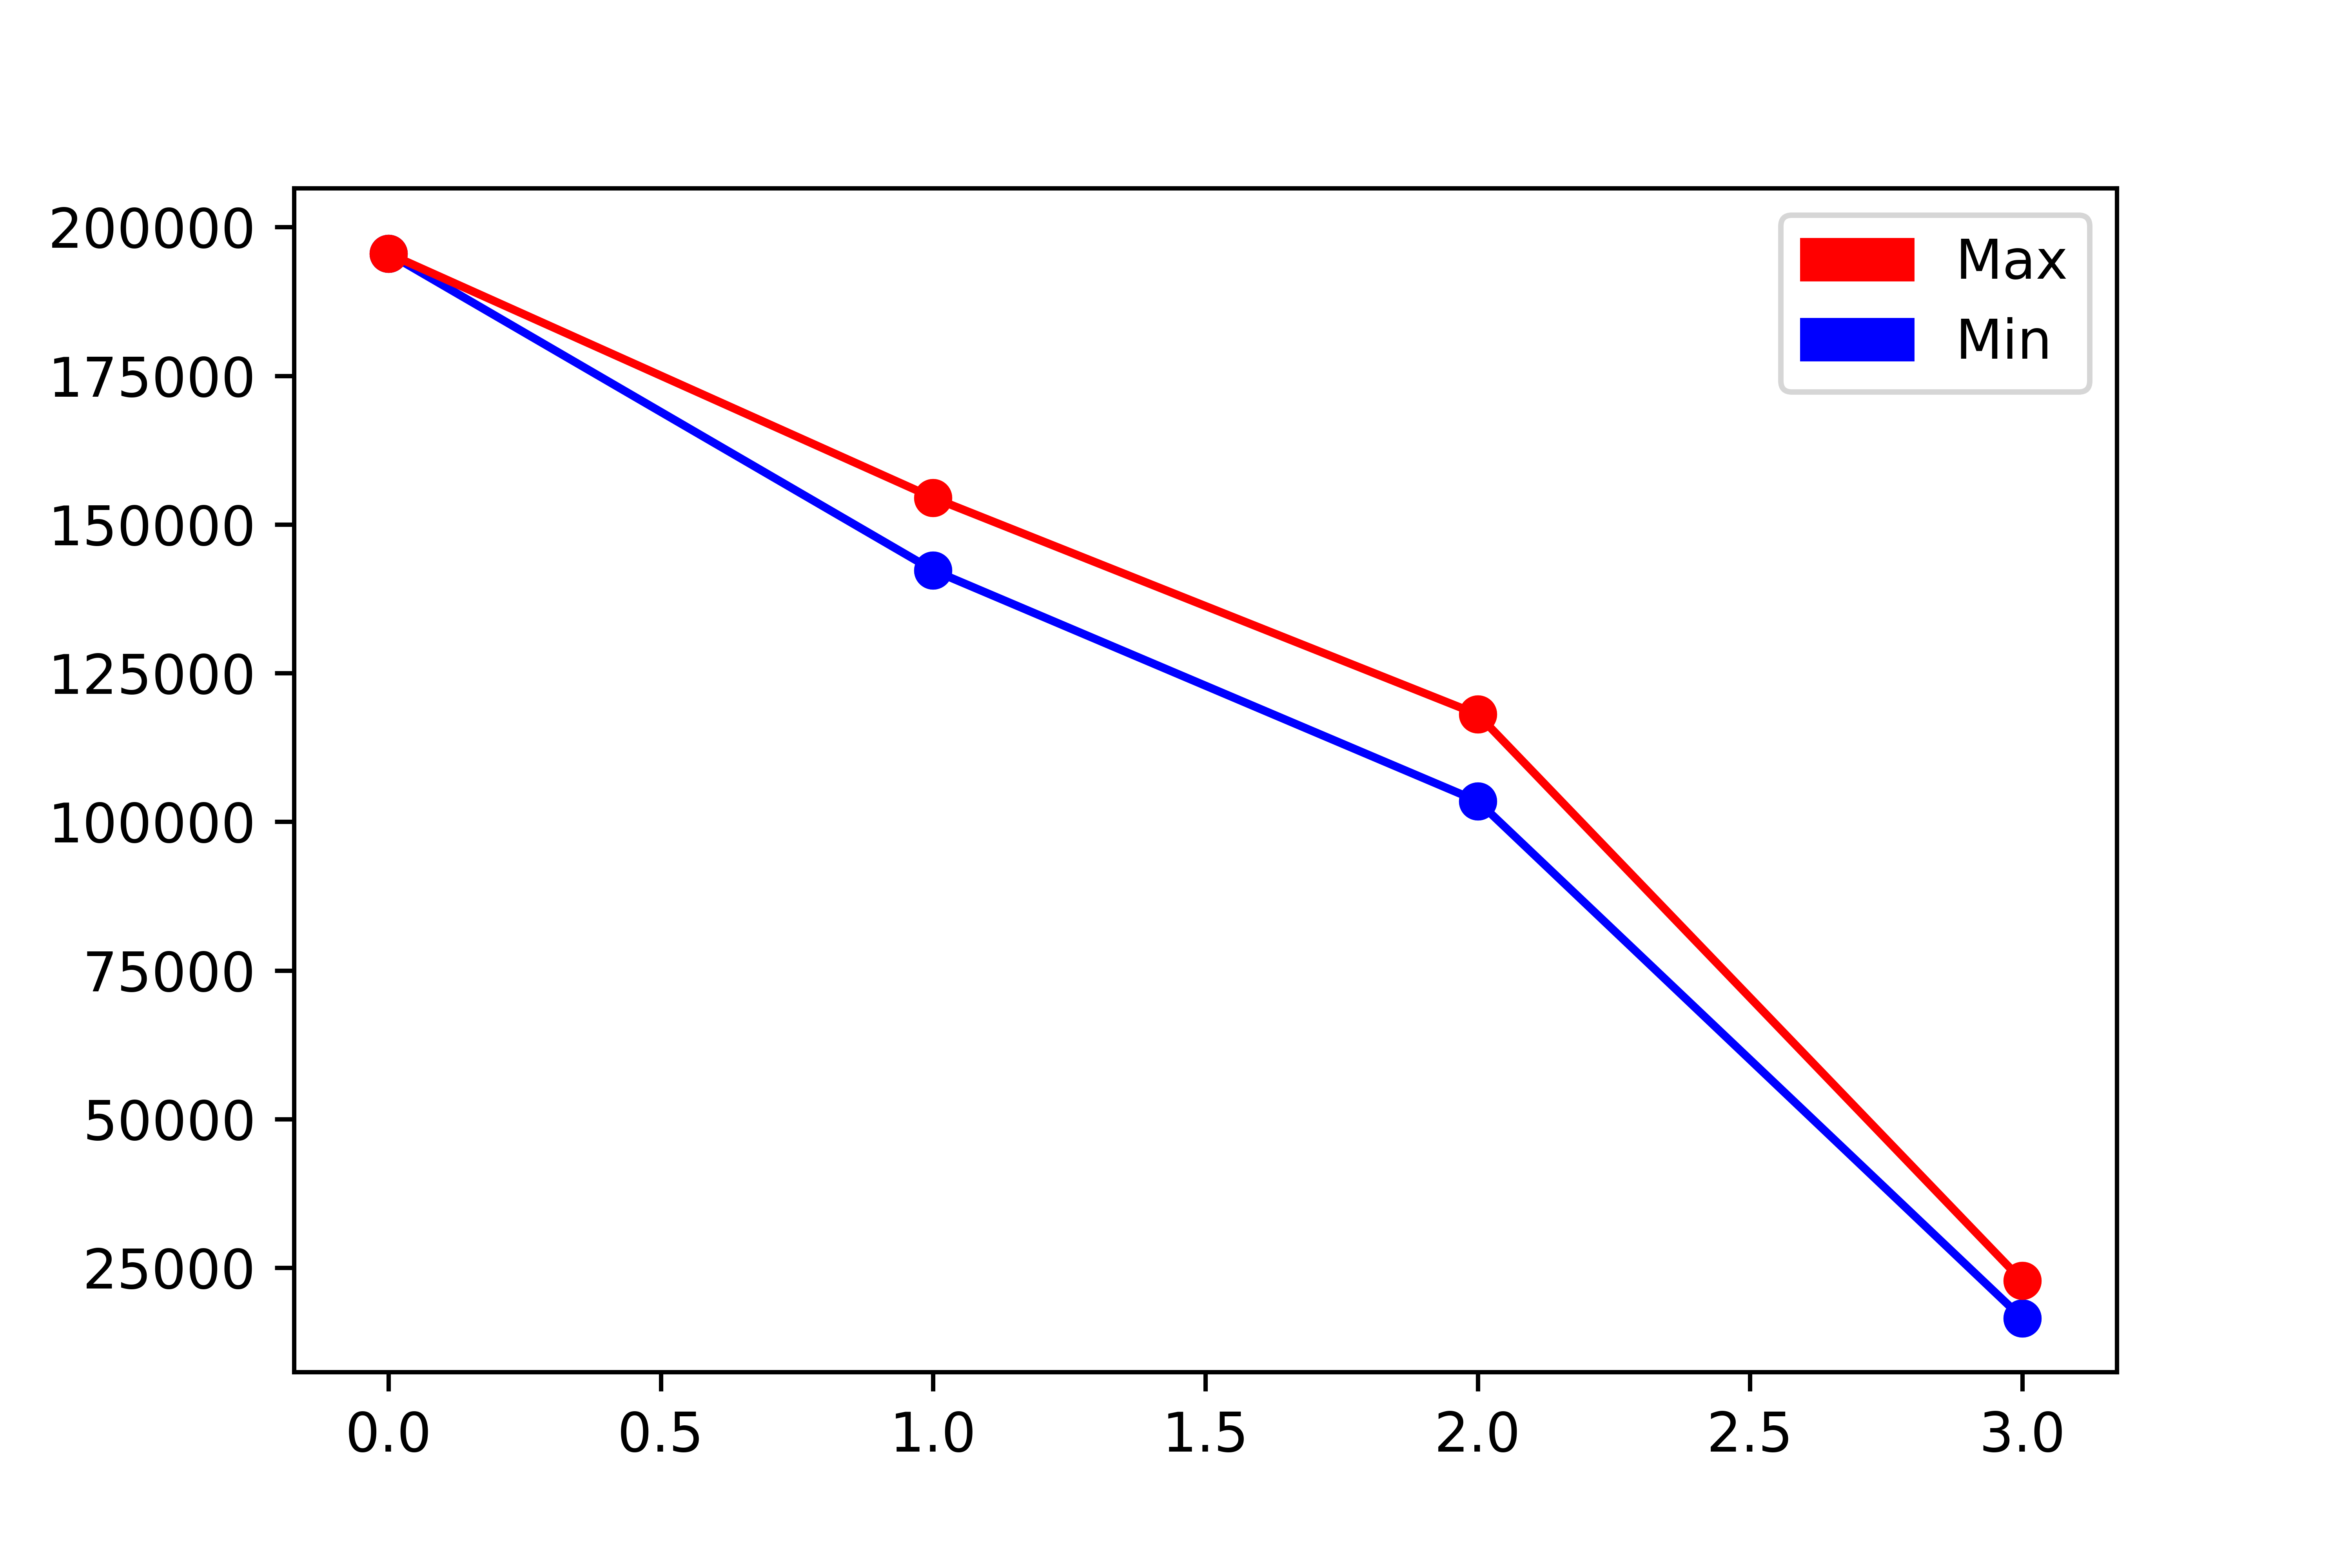
\includegraphics[width=0.80\textwidth]{effectifs_cumules_durees_maximales_minimales_qd_ib_NaN_traite_comme_chgmt_grade.png} 
\end{figure}
\begin{minipage}{15cm}
	\footnotesize
	\textsc{Population:} 195 540 agents (statut d'ambiguité). Agents qui changent au moins une fois de grade entre 2007 et 2011 et qui ne sont pas classés ambigüs en 2007. \\
	\textsc{Lecture:} Environ 150 000 agents ont une durée prédite passée dans le grade minimale au moins égale à 1 an. Un peu plus de 150 000 agents ont une durée prédite maximale passée dans le grade égale à 1 ans (i.e ils passent 0 ou 1 an dans leur grade).
\end{minipage}


Problème de changement de grille à retardement :
\begin{figure}[H] 
	\caption{Histogramme des durées maximales et durées minimales prédites passées dans le grade.}
	\label{transit1} 
	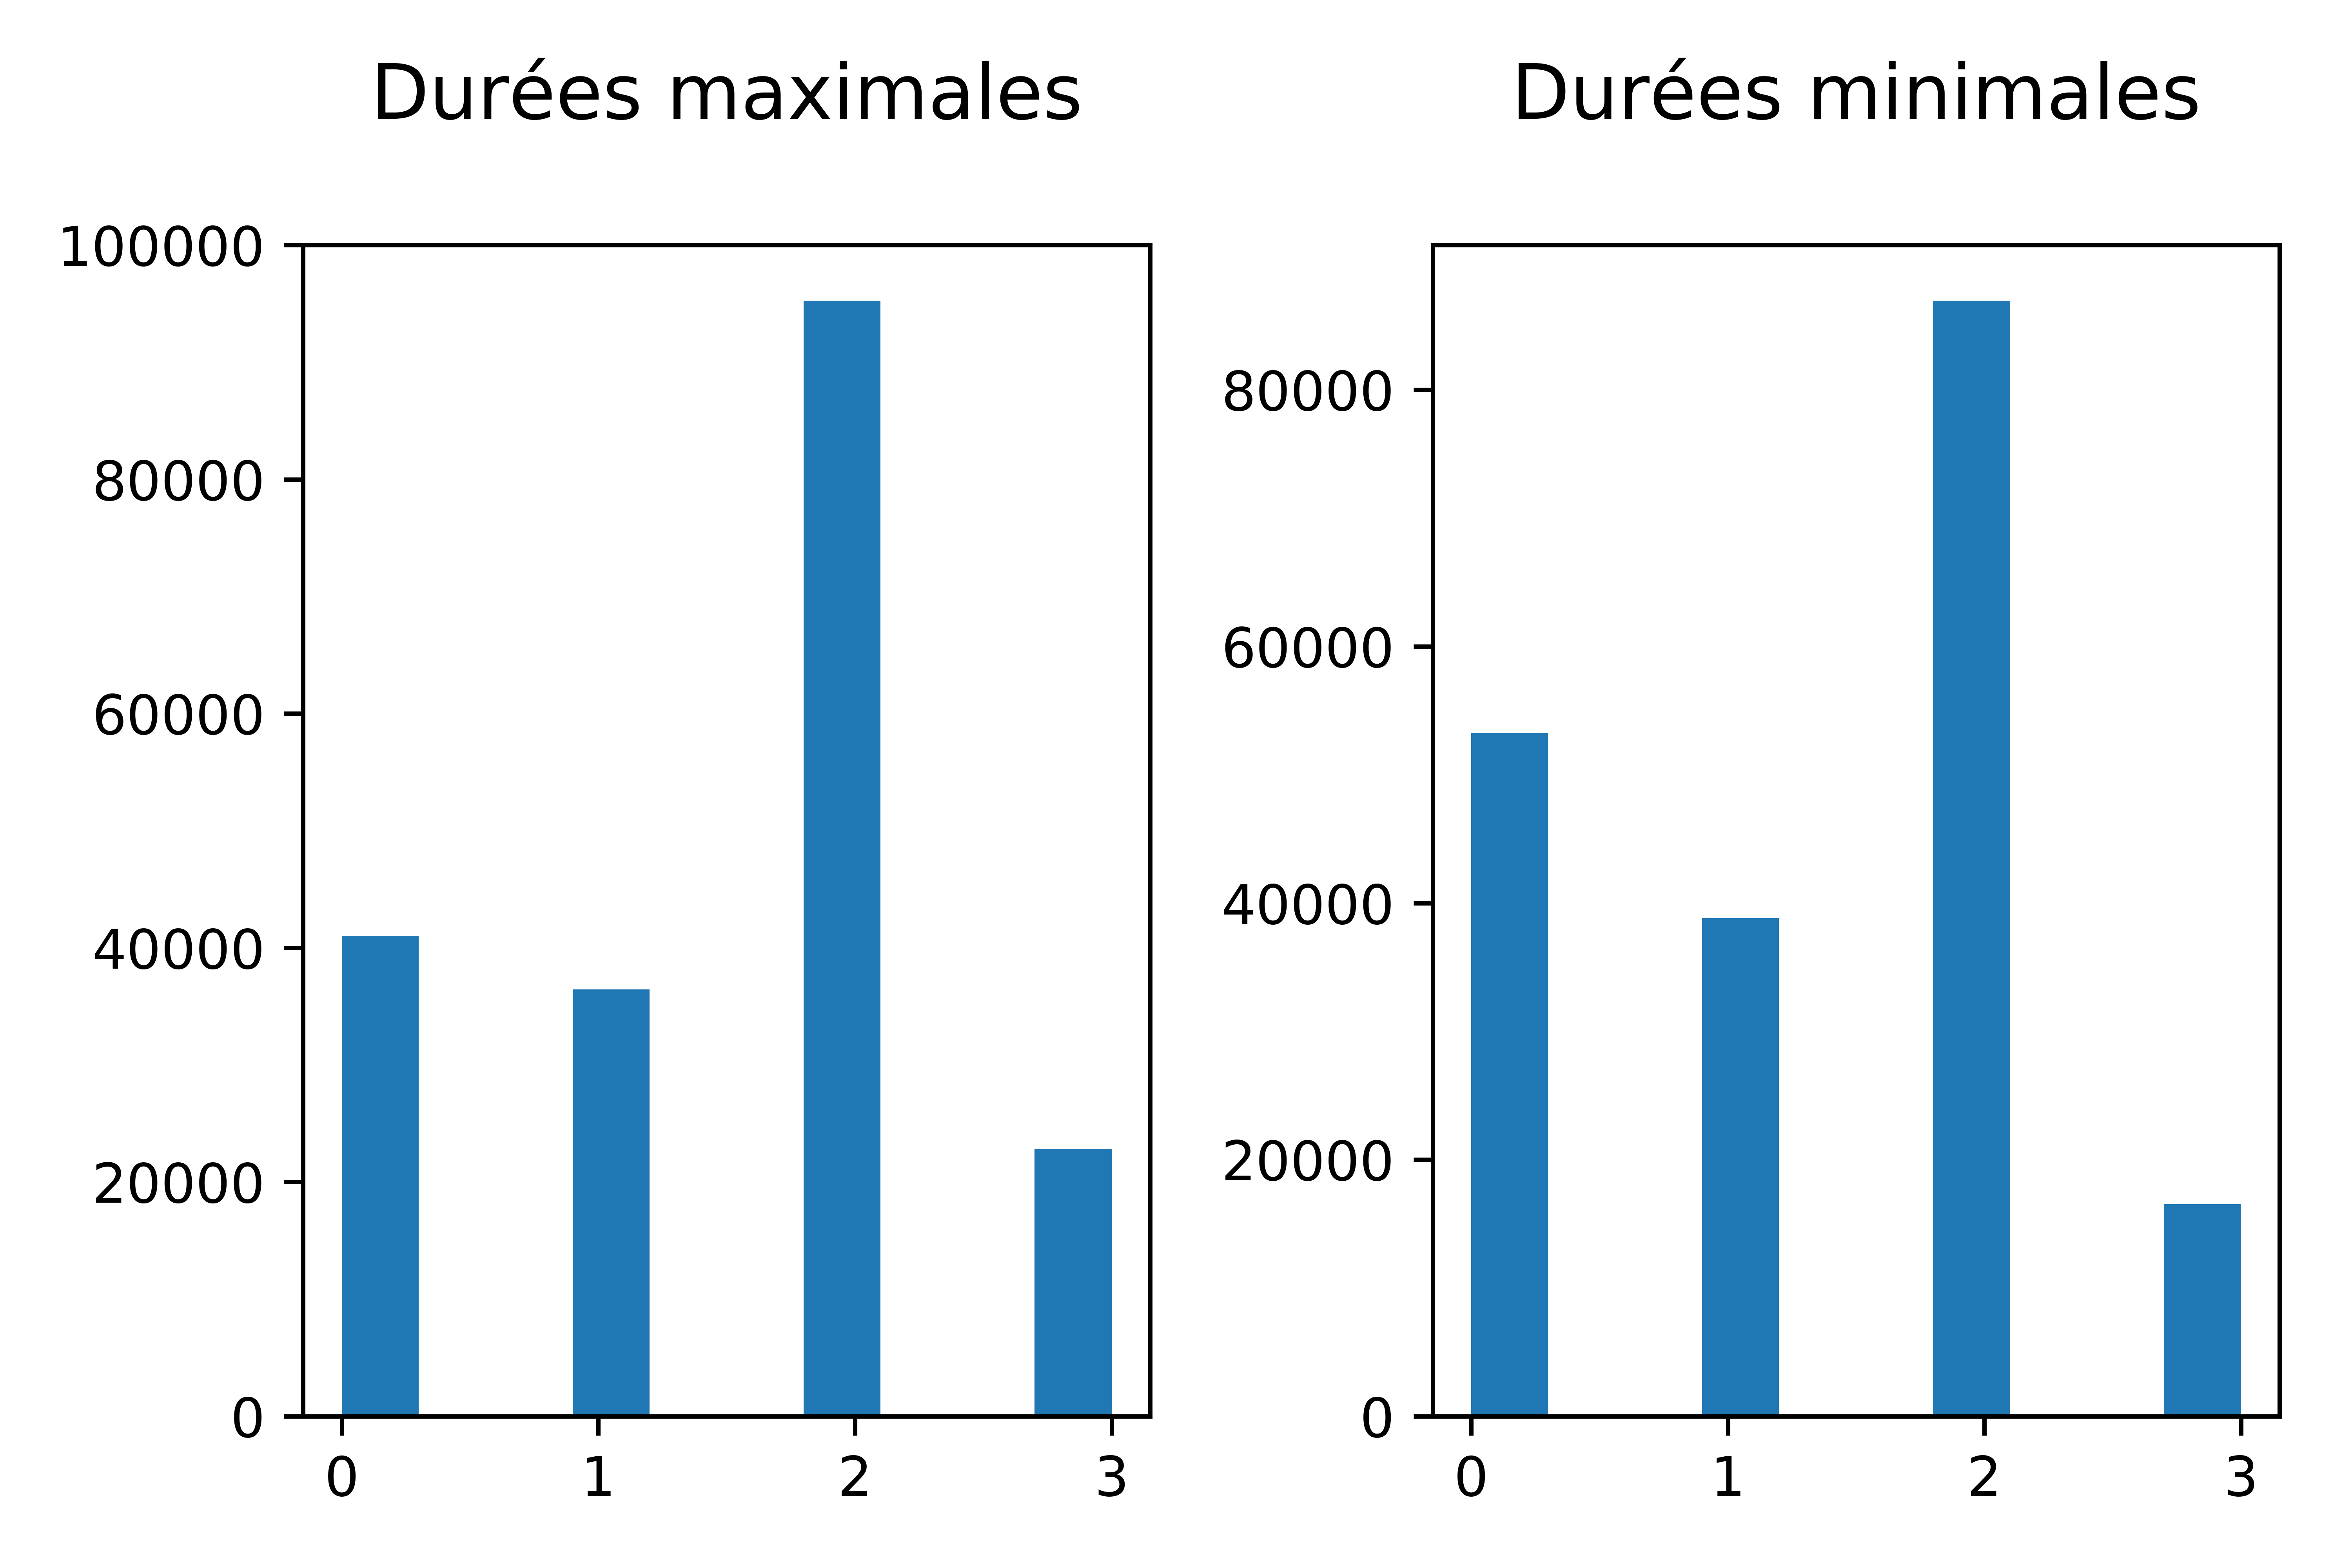
\includegraphics[width=0.70\textwidth]{histogramme_durees_maximales_minimales_qd_ib_NaN_traite_comme_chgmt_grade.png} 
\end{figure}
\begin{minipage}{15cm}
	\footnotesize
	\textsc{Population:} 195 540 agents. Agents qui changent au moins une fois de grade entre 2007 et 2011 et qui ne sont pas classés ambigüs en 2007.\\
	\textsc{Lecture:} Il y a 40 000 agents pour lesquelles la durée maximale prédite passée dans le grade est de 0.
\end{minipage}

\begin{figure}[H] 
	\caption{}
	\label{transit1} 
	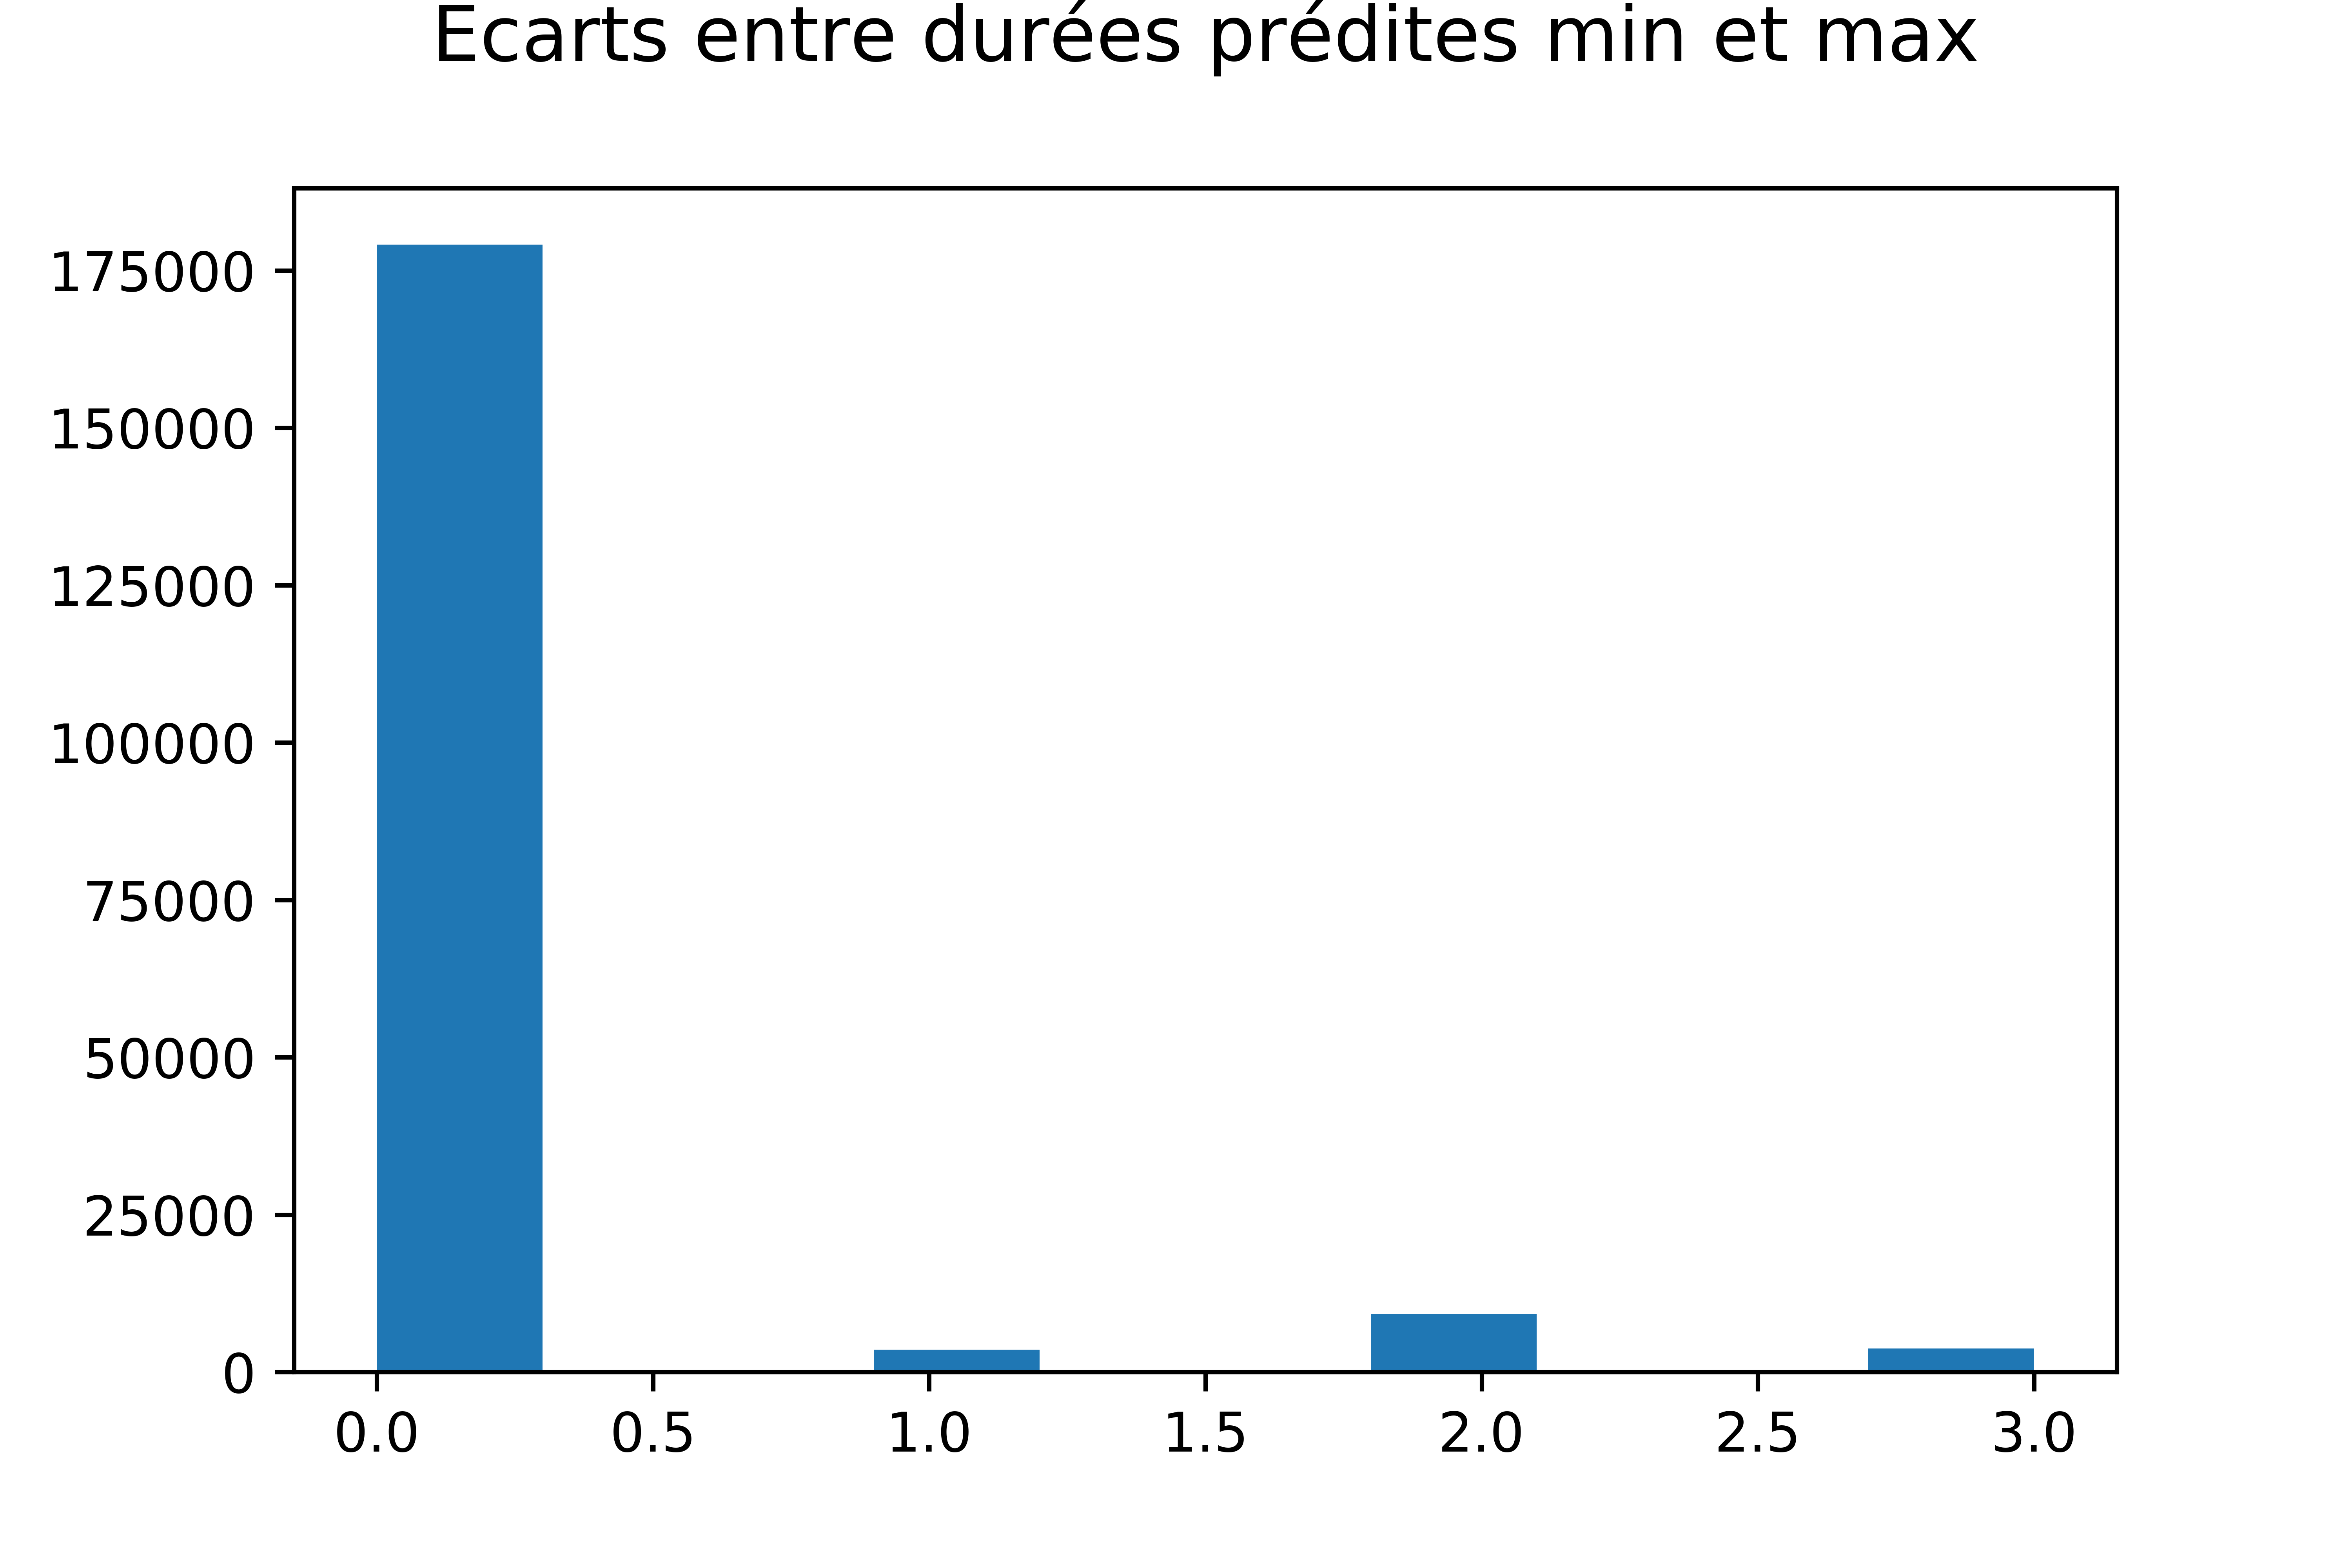
\includegraphics[width=0.70\textwidth]{histogramme_des_ecarts_qd_ib_NaN_traite_comme_chgmt_grade.png} 
\end{figure}
\begin{minipage}{15cm}
	\footnotesize
	\textsc{Population:} 195 540 agents. Agents qui changent au moins une fois de grade entre 2007 et 2011 et qui ne sont pas classés ambigüs en 2007.\\
	\textsc{Lecture:} Il y a 175 000 agents pour lesquels la durée min prédite est égale à la durée max prédite. C'est différent de la question de l'ambiguité car on peut avoir de gros écarts entre durées prédites min et max et la certitude de cette écart ou l'incertitude sur une des bornes.
\end{minipage}
\bigskip

\begin{table}
	\caption{Tabulation de l'ambiguité et des écarts de prédiction}
\begin{tabular}{lrrrr}
	\toprule
	ecart &     0.0 &   1.0 &   2.0 &   3.0 \\
	ambig &         &       &       &       \\
	\midrule
	False                    &  179103 &  3208 &  8120 &  3365 \\
	True                     &       0 &   319 &  1066 &   359 \\
	\bottomrule
\end{tabular}
\end{table}

\pagebreak
\subsection{Types d'information disponible}


\begin{tabular}{lllrrr}
	\toprule
	{} & ambig sur min & ambig sur max &  min &  max &   nombre d'agents \\
	\midrule
	1 &           False &           False &                           2.0 &                           2.0 &  664596 \\
	2 &           False &           False &                           0.0 &                           0.0 &  243531 \\
	3 &           False &           False &                           1.0 &                           1.0 &  223092 \\
	4 &           False &           False &                           3.0 &                           3.0 &  119637 \\
	5 &            True &           False &                           0.0 &                           2.0 &   49509 \\
	6 &            True &           False &                           0.0 &                           3.0 &   25794 \\
	7 &            True &           False &                           1.0 &                           3.0 &   17946 \\
	8 &            True &           False &                           1.0 &                           2.0 &   10881 \\
	9 &            True &           False &                           0.0 &                           1.0 &    8154 \\
	10 &            True &           False &                           2.0 &                           3.0 &    2502 \\
	\bottomrule
\end{tabular}

\begin{itemize}
	\item Dans les 4 premiers cas, on est certain que les agents ont déjà passé 2, 0 1 et 3 ans respectivement dans leur grade en 2011.
	\item Dans les 6 cas suivants et pour le 11ème cas, on sait pour sûr que les agents sont restés dans leur grade 2, 3, 3, 2, 1 et 3 ans respectivement au maximum, mais qu'ils sont peut-être restés moins longtemps (0, 0, 1, 1 ou 0 années).
\end{itemize}

\begin{tabular}{lrrllr}
	\toprule
	{} &  min  &  max & ambig min & ambig max &  ident \\
	\midrule
	0  &                           0.0 &                           0.0 &           False &           False &  26732 \\
	7  &                           1.0 &                           1.0 &           False &           False &  23607 \\
	17 &                           3.0 &                           3.0 &           False &           False &  22844 \\
	13 &                           2.0 &                           2.0 &           False &           False &  18774 \\
	3  &                           0.0 &                           2.0 &            True &           False &   4034 \\
	5  &                           0.0 &                           3.0 &            True &           False &   3078 \\
	6  &                           0.0 &                           3.0 &            True &            True &   2904 \\
	15 &                           2.0 &                           3.0 &            True &           False &   2488 \\
	16 &                           2.0 &                           3.0 &            True &            True &   2460 \\
	11 &                           1.0 &                           3.0 &            True &           False &   2140 \\
	18 &                           3.0 &                           3.0 &            True &            True &   1565 \\
	12 &                           1.0 &                           3.0 &            True &            True &   1079 \\
	1  &                           0.0 &                           1.0 &            True &           False &    841 \\
	14 &                           2.0 &                           2.0 &            True &            True &    841 \\
	9  &                           1.0 &                           2.0 &            True &           False &    520 \\
	4  &                           0.0 &                           2.0 &            True &            True &    466 \\
	2  &                           0.0 &                           1.0 &            True &            True &     63 \\
	8  &                           1.0 &                           1.0 &            True &            True &     41 \\
	10 &                           1.0 &                           2.0 &            True &            True &     25 \\
	\bottomrule
\end{tabular}
\section{Idées}

- Transitions de corps

\end{document}